\begin{savequote}[45mm]
\ascii{Any fool can write code that a computer can understand. Good programmers write code that humans can understand.}
\qauthor{\ascii{- Martin Flower}}
\end{savequote}

\chapter{实现xUnit} 
\label{ch:ice-breaker}

\begin{content}

\end{content}

\section{提出问题}
	
\begin{content}

\subsection{xUnit架构}

\subsection{接口设计}

使用\ascii{C++}描述\ascii{xUnit}的样例,相对于\ascii{Google Test},此处做了如下几个方面的革新。

\begin{enum}
  \eitem{\ascii{在同一个类域内,使得TEST与SETUP/TEARDOWN关系更加紧密;}}
  \eitem{\ascii{使用字符串描述用例;}}
  \eitem{\ascii{避免setUp, SetUp, setup大小写混用导致的错误。}}
\end{enum}


\begin{leftbar}
 \begin{c++}
#include <statck>
#include "mars/mars.h"

FIXTURE(StackSpec) {
  std::stack<int> v;   

  SETUP {
    v.push(1);
  }

  TEST("top element") {
    ASSERT_EQ(1, v.top());
  }
 
  TEARDOWN {
    v.pop();
  }
}; 
 \end{c++}
\end{leftbar}

\end{content}

\section{破冰之旅}

\begin{content}

\subsection{环境准备}

创建一个项目并命名为\ascii{mars},然后在项目的顶层目录初始化一个\ascii{git}库。

\begin{leftbar}
 \begin{c++}[caption={\ttfamily{初始化git库}}] 
$ git init 
 \end{c++}
\end{leftbar}  

\subsubsection{项目组织}

项目目录结构如下。

\begin{leftbar}
 \begin{c++}[caption={\ttfamily{项目组织}}]
mars
├── build
├── CMakeLists.txt
├── include
│   └── mars
├── src
│   ├── CMakeLists.txt
│   └── mars
└── test
    ├── CMakeLists.txt
    └── mars
 \end{c++}
\end{leftbar}

\subsubsection{CMakeList实现}

主控的\ascii{CMakeLists.txt}内容如下:

\begin{leftbar}
 \begin{c++}[caption={\ttfamily{CMakeLists.txt}}]
project(mars)                                                                                  
cmake_minimum_required(VERSION 3.10)

set(CMAKE_CXX_FLAGS "${CMAKE_CXX_FLAGS} -std=c++14")

include_directories("${CMAKE_CURRENT_SOURCE_DIR}/include")

add_subdirectory(src)
add_subdirectory(test)
 \end{c++}
\end{leftbar}

\ascii{src/CMakeLists.txt}完成\ascii{mars}库的构建。

\begin{leftbar}
 \begin{c++}[caption={\ttfamily{src/CMakeLists.txt}}]
file(GLOB_RECURSE all_files *.cc)
add_library(mars STATIC ${all_files})
 \end{c++}
\end{leftbar}

\ascii{test/CMakeLists.txt}完成\ascii{mars-test}应用程序的构建,执行\ascii{mars}的测试用例。

\begin{leftbar}
 \begin{c++}[caption={\ttfamily{test/CMakeLists.txt}}]
file(GLOB_RECURSE all_files *.cc)
add_executable(mars-test ${all_files})
target_link_libraries(mars-test mars gtest gtest_main pthread)
 \end{c++}
\end{leftbar}

提交代码。

\begin{leftbar}
 \begin{c++}[caption={\ttfamily{提交代码}}] 
$ git add -A .
$ git commit -m"setup project"
 \end{c++}
\end{leftbar}  

\subsection{起航}

万事开头难,第一个用例跑起来并不容易,此处设计实现了一个最简单的测试用例。当用户新增一个用例时,框架需要具有良好的扩展性,需要很方便地支持用户的测试用例的设计。在面向对象设计中,通常通过扩展子类实现开放封闭的设计原则。

\begin{leftbar}
 \begin{c++}[caption={\ttfamily{test/mars/core/TestCaseSpec.cc}}]
#include <gtest/gtest.h>
#include "mars/core/TestCase.h"

namespace {
  struct SimpleTest : TestCase {
    bool wasRun = false;

  private:
    void run() override {
      wasRun = true;
    }
  };

  void run(TestCase& test) {
    test.run();
  }
}

TEST(SimpleTest, make_sure_test_case_can_run_normally) {
  SimpleTest test;
  run(test);

  ASSERT_TRUE(test.wasRun);
}
 \end{c++}
\end{leftbar}

\subsubsection{通过编译}

此处引入了多态技术,当\ascii{TestCase::run}启动运行时,将在运行时调用覆写的\ascii{SimpleTest::run},实现自定义测试用例的执行。

\begin{leftbar}
 \begin{c++}[caption={\ttfamily{include/mars/core/TestCase.h}}]
struct TestCase {
  virtual ~TestCase() {}
  virtual void run() = 0;
};
  \end{c++}
\end{leftbar}

\subsubsection{通过链接}

创建了一个空的\ascii{TestCase.cc}文件,仅为了\ascii{libmars.a}不为空,保证链接成功。

\begin{leftbar}
 \begin{c++}[caption={\ttfamily{src/mars/core/TestCase.cc}}]
#include "mars/core/TestCase.h"
 \end{c++}
\end{leftbar}

\subsubsection{通过测试}

在\ascii{build}临时目录中,使用\ascii{cmake}构建工程。

\begin{leftbar}
 \begin{c++}[caption={\ttfamily{构建工程}}]
$ mkdir -p build && cd build
$ cmake ..
$ make
 \end{c++}
\end{leftbar}

运行测试。

\begin{leftbar}
 \begin{c++}[caption={\ttfamily{运行测试}}]
$ test/mars-test
Running main() from gtest_main.cc
[==========] Running 1 test from 1 test case.
[----------] Global test environment set-up.
[----------] 1 test from SimpleTest
[ RUN      ] SimpleTest.make_sure_test_case_can_run_normally
[       OK ] SimpleTest.make_sure_test_case_can_run_normally (0 ms)
[----------] 1 test from SimpleTest (0 ms total)

[----------] Global test environment tear-down
[==========] 1 test from 1 test case ran. (1 ms total)
[  PASSED  ] 1 test.
 \end{c++}
\end{leftbar}

\subsubsection{提交代码}

每当通过测试后,立即提交代码到\ascii{Git}库。

\begin{leftbar}
 \begin{c++}[caption={\ttfamily{提交代码}}]
$ git add -A .
$ git commit -m"pass first test case"
 \end{c++}
\end{leftbar}

\end{content}

\section{算法骨架}

\begin{content}

一般地,在执行测试前需要预置\ascii{setUp}实施测试环境的初始化工作,完成资源的准备。对既有的用例实施重构。

\subsection{前置}

\begin{leftbar}
 \begin{c++}[caption={\ttfamily{test/mars/core/TestCaseSpec.cc}}]
#include <gtest/gtest.h>
#include "mars/core/TestCase.h"

namespace {
  struct SimpleTest : TestCase {
    bool wasSetUp = false;
    bool wasRun = false;

  private:
    void setUp() override {
      wasSetUp = true;
    }

    void runTest() override {
      wasRun = true;
    }
  };
}

TEST(SimpleTest, make_sure_test_case_can_run_normally) {
  SimpleTest test;
  test.run();

  ASSERT_TRUE(test.wasSetUp);
  ASSERT_TRUE(test.wasRun);
}
 \end{c++}
\end{leftbar}

\subsubsection{通过编译}

重构\ascii{TestCase},仅公开\ascii{run}方法,并移除运行时多态的特性,它负责用例执行的运行时的算法骨架。搬迁运行时多态行为至私有的两个虚函数,用户根据自己的场景定制\ascii{setUp}与\ascii{runTest},分别完成测试准备,及其测试执行。

\begin{leftbar}
 \begin{c++}[caption={\ttfamily{include/mars/core/TestCase.h}}]
struct TestCase {
  virtual ~TestCase() {}

  void run();

private:
  virtual void setUp() {}
  virtual void runTest() {}
};
  \end{c++}
\end{leftbar}

\subsubsection{通过测试}

实现\ascii{TestCase::run}的主体逻辑。

\begin{leftbar}
 \begin{c++}[caption={\ttfamily{src/mars/core/TestCase.cc}}]
#include "mars/core/TestCase.h"

void TestCase::run() {
  setUp();
  runTest();
}

 \end{c++}
\end{leftbar}

测试通过。

\subsection{后置}

同理,测试执行后使用\ascii{tearDown}完成现场清理,释放资源。用户通过定制私有的虚函数\ascii{tearDown}完成此功能。

\begin{leftbar}
 \begin{c++}[caption={\ttfamily{test/mars/core/TestCaseSpec.cc}}]
#include <gtest/gtest.h>
#include "mars/core/TestCase.h"

namespace {
  struct SimpleTest : TestCase {
    bool wasSetUp = false;
    bool wasRun = false;
    bool wasTearDown = false;

  private:
    void setUp() override {
      wasSetUp = true;
    }

    void runTest() override {
      wasRun = true;
    }

    void tearDown() override {
      wasTearDown = true;
    }
  };
}

TEST(SimpleTest, make_sure_test_case_can_run_normally) {
  SimpleTest test;
  test.run();

  ASSERT_TRUE(test.wasSetUp);
  ASSERT_TRUE(test.wasRun);
  ASSERT_TRUE(test.wasTearDown);  
}
 \end{c++}
\end{leftbar}

\subsubsection{通过编译}

当用例执行完成后,\ascii{TestCase::tearDown}负责清理现场。

\begin{leftbar}
 \begin{c++}[caption={\ttfamily{include/mars/core/TestCase.h}}]
struct TestCase {
  virtual ~TestCase() {}

  void run();

private:
  virtual void setUp() {}
  virtual void runTest() {}
  virtual void tearDown() {}
};
  \end{c++}
\end{leftbar}

\subsubsection{通过测试}

至此,完成了运行一个用例的主干逻辑,但缺乏异常处理机制,留待后续处理。

\begin{leftbar}
 \begin{c++}[caption={\ttfamily{src/mars/core/TestCase.cc}}]
#include "mars/core/TestCase.h"

void TestCase::run() {
  setUp();
  runTest();
  tearDown();
}
 \end{c++}
\end{leftbar}

\begin{figure}[H]
\centering
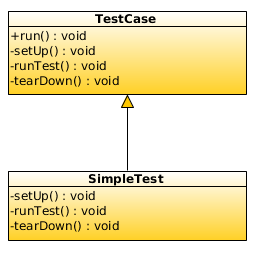
\includegraphics[width=0.4\textwidth]{figures/xunit/simple-test.png}
\caption{模板方法:定义算法骨架}
 \label{fig:simple-test}
\end{figure}

\end{content}

\section{隐式树}

\begin{content}

如果每个用例都需要手动地执行\ascii{run},显得极其笨拙。可以将一堆测试用例打包,用一个简单的\ascii{for}循环依次执行每个用例。

\subsection{测试套件}

为了确定每个\ascii{TestCase}都被执行,可以简单定制一个计数器\ascii{num},用例执行后,断言已运行用例的数目。

\begin{leftbar}
 \begin{c++}[caption={\ttfamily{test/mars/core/TestSuiteSpec.cc}}]
#include <gtest/gtest.h>
#include "mars/core/TestCase.h"
#include "mars/core/TestSuite.h"

namespace {
  int num = 0;

  struct FooTest : TestCase {
  private:
    void runTest() override {
      num++;
    }
  };
}

TEST(TestSuite, run_multi_test_cases_using_test_suite) {
  TestSuite suite;
  suite.add(new FooTest);
  suite.add(new FooTest);

  suite.run();

  ASSERT_EQ(2, num);
}
 \end{c++}
\end{leftbar}

\subsubsection{通过编译}

为了快速通过编译,创建\ascii{TestSuite}的头文件。

\begin{leftbar}
 \begin{c++}[caption={\ttfamily{include/mars/core/TestSuite.h}}]
#include <vector>

struct TestCase;

struct TestSuite {
  void add(TestCase* test);
  void run();

private:
  std::vector<TestCase*> tests;
};
 \end{c++}
\end{leftbar}

\subsubsection{通过测试}

为了通过测试,可以快速实现\ascii{TestSuite::run}的逻辑。

\begin{leftbar}
 \begin{c++}[caption={\ttfamily{src/mars/core/TestSuite.cc}}]
#include "mars/core/TestSuite.h"
#include "mars/core/TestCase.h"

void TestSuite::add(TestCase* test) {
  tests.push_back(test);
}

void TestSuite::run() {
  for (auto test : tests) {
    test->run();
  }
}
 \end{c++}
\end{leftbar}

\subsubsection{内存泄露}

\ascii{TestSuite}持有若干\ascii{TestCase}实例,引入析构函数释放动态创建并添加至\ascii{TestSuite}的所有\ascii{TestCase}实例。

\begin{leftbar}
 \begin{c++}[caption={\ttfamily{include/mars/core/TestSuite.h}}]
#include <vector>

struct TestCase;

struct TestSuite {
  ~TestSuite();

  void add(TestCase* test);
  void run();

private:
  std::vector<TestCase*> tests;
};
 \end{c++}
\end{leftbar}

实现析构函数,释放动态内存。

\begin{leftbar}
 \begin{c++}[caption={\ttfamily{src/mars/core/TestSuite.cc}}]
#include "mars/core/TestSuite.h"
#include "mars/core/TestCase.h"

void TestSuite::add(TestCase* test) {
  tests.push_back(test);
}

TestSuite::~TestSuite() {
  for (auto test : tests) {
    delete test;
  }
}

void TestSuite::run() {
  for (auto test : tests) {
    test->run();
  }
}
 \end{c++}
\end{leftbar}

\subsubsection{消除重复}

为了消除析构函数与\ascii{run}之间的重复代码,提取一个公共的\ascii{foreach}函数。注意,不要在头文件直接实现该模板函数,最小化编译时的依赖。

\begin{leftbar}
 \begin{c++}[caption={\ttfamily{include/mars/core/TestSuite.h}}]
#include <vector>

struct TestCase;

struct TestSuite {
  ~TestSuite();

  void add(TestCase* test);
  void run();

private:
  template <typename F>
  void foreach(F f) const;

private:
  std::vector<TestCase*> tests;
};
 \end{c++}
\end{leftbar}

因此,设计得到两个独立变化的方向。

\begin{enum}
  \eitem{\ascii{迭代算法:因存储结构变化而变化(目前实现为线性列表,不排除将来实现为map);}}
  \eitem{\ascii{处理算子:存在删除,计数,运行等操作。}}
\end{enum}

可以使用\ascii{Lambda}表达式定制各种算子,实现差异化配置,实现对迭代算法的高度复用。

\begin{leftbar}
 \begin{c++}[caption={\ttfamily{src/mars/core/TestSuite.cc}}]
#include "mars/core/TestSuite.h"
#include "mars/core/TestCase.h"

void TestSuite::add(TestCase* test) {
  tests.push_back(test);
}

template <typename F>
inline void TestSuite::foreach(F f) const {
  for (auto test : tests) {
    f(test);
  }
}

TestSuite::~TestSuite() {
  foreach([](auto test) {
    delete test;
  });
}

void TestSuite::run() {
  foreach([](auto test) {
    test->run();
  });
}
 \end{c++}
\end{leftbar}

\subsection{嵌套结构}

为了实现更好的可扩展性,\ascii{TestSuite}不仅能打包\ascii{TestCase}实例,也应该能够打包更小的\ascii{TestSuite}的子实例,实现隐式的树结构。


\begin{figure}[H]
\centering
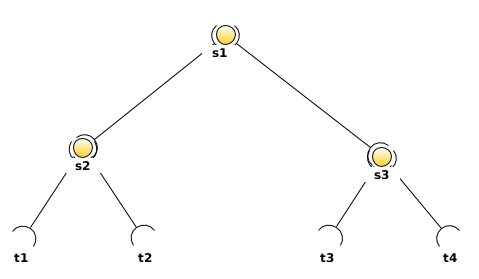
\includegraphics[width=0.8\textwidth]{figures/xunit/test-tree-example.png}
\caption{用例树:TestSuite(s1, s2, s3),TestCase(t1,t2,t3,t4)}
 \label{fig:simple-test}
\end{figure}

\subsubsection{测试依赖}

为了能够添加更多的用例,需要对计数器\ascii{num}实施初始化。当执行用例时,确保\ascii{num}被初始化为\ascii{0};否则测试用例之间存在数据脏写的错误依赖。另外,此处没有直接调用\ascii{TestSuite::run},而是使用更为抽象的\ascii{Test::run},测试装置将更加稳定。

在实现\ascii{TestSuiteSpec::run}时,显式地使用域限定符\ascii{::Test},避免与\ascii{testing::Test}产生二义性而导致编译失败。

\begin{leftbar}
 \begin{c++}[caption={\ttfamily{test/mars/core/TestSuiteSpec.cc}}]
#include <gtest/gtest.h>
#include "mars/core/TestCase.h"
#include "mars/core/TestSuite.h"

namespace {
  int num = 0;

  struct FooTest : TestCase {
  private:
    void runTest() override {
      num++;
    }
  };

  struct TestSuiteSpec : testing::Test {
  private:
    void SetUp() override {
      num = 0;  // IMPORTANT: reset counter.
    }

  protected:
    void run(::Test& test) {
      test.run();
    }
  };
}

TEST_F(TestSuiteSpec, package_multi_test_cases_into_test_suite) {
  TestSuite suite;
  suite.add(new FooTest);
  suite.add(new FooTest);

  run(suite);

  ASSERT_EQ(2, num);
}

TEST_F(TestSuiteSpec, package_sub_test_suite_into_outter_test_suite) {
  auto inner = new TestSuite;
  inner->add(new FooTest);

  TestSuite outter;
  outter.add(new FooTest);
  outter.add(inner);

  run(outter);

  ASSERT_EQ(2, num);
}
 \end{c++}
\end{leftbar}

此时,第二个测试用例编译失败。

\subsubsection{提取抽象}

通过提取\ascii{TestCase}与\ascii{TestSuite}的共同抽象\ascii{Test},从而使得用例的组织更加灵活。

\begin{leftbar}
 \begin{c++}[caption={\ttfamily{include/mars/core/Test.h}}]
struct Test {
  virtual ~Test() {}
  virtual void run() = 0;
};
 \end{c++}
\end{leftbar}

\subsubsection{重构TestCase}

重构\ascii{TestCase},所有显式声明的成员函数都是\ascii{private}。尤其关注被覆写的\ascii{TestCase::run},被显式地声明为\ascii{private},逼迫用户使用抽象接口\ascii{Test::run},而“面向接口编程”是一种良好的\ascii{OO}设计原则。

\begin{leftbar}
 \begin{c++}[caption={\ttfamily{include/mars/core/TestCase.h}}]
#include "mars/core/Test.h"

struct TestCase : Test {
private:
  void run() override;

private:
  virtual void setUp() {}
  virtual void runTest() {}
  virtual void tearDown() {}
};
 \end{c++}
\end{leftbar}

\subsubsection{重构TestSuite}

同理,\ascii{TestSuite}也应该被重构使用\ascii{Test}的抽象类型,而非使用\ascii{TestCase}的具体类型。

\begin{leftbar}
 \begin{c++}[caption={\ttfamily{include/mars/core/TestSuite.h}}]
#include <vector>
#include "mars/core/Test.h"

struct TestSuite : Test {
  ~TestSuite();
  void add(Test* test);

private:
  void run() override;

private:
  template <typename F>
  void foreach(F f) const;

private:
  std::vector<Test*> tests;
};
 \end{c++}
\end{leftbar}

同理,\ascii{TestSuite}的实现也应该使用\ascii{Test}的抽象类型。幸运的是,原来使用\ascii{auto}的自动类型推演,实现文件仅需要修改\ascii{TestSuite::add}函数签名便可以通过测试了。

\begin{leftbar}
 \begin{c++}[caption={\ttfamily{src/mars/core/TestSuite.cc}}]
#include "mars/core/TestSuite.h"

void TestSuite::add(Test* test) {
  tests.push_back(test);
}

template <typename F>
inline void TestSuite::foreach(F f) const {
  for (auto test : tests) {
    f(test);
  }
}

TestSuite::~TestSuite() {
  foreach([](auto test) {
    delete test;
  });
}

void TestSuite::run() {
  foreach([](auto test) {
    test->run();
  });
}
 \end{c++}
\end{leftbar}

通过\ascii{Test, TestCase, TestSuite},可以方便地组合复杂树形结构的用例图。

\begin{figure}[H]
\centering
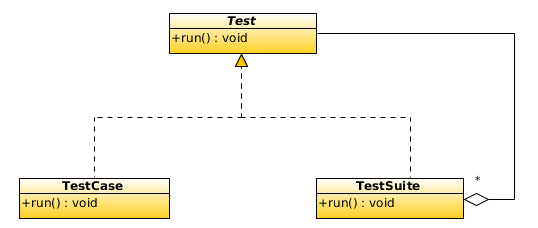
\includegraphics[width=0.8\textwidth]{figures/xunit/test-tree.png}
\caption{组合:构建隐式树}
 \label{fig:test-tree}
\end{figure}

\subsection{命名用例}

可以给每个\ascii{TestCase, TestSuite}命名,方便后期用例的定位与调试。

\begin{leftbar}
 \begin{c++}[caption={\ttfamily{test/mars/core/TestSuiteSpec.cc}}]
#include <gtest/gtest.h>
#include "mars/core/TestCase.h"

namespace {
  void assertName(const Test& test, const char* expected) {
    ASSERT_EQ(std::string(expected), test.getName());
  }
}

TEST(NamedTestCase, named_test_case) {
  assertName(TestCase("test case1"), "test case1");
}
 \end{c++}
\end{leftbar}

\subsubsection{通过测试}

首先,增加抽象接口\ascii{Test::getName}。

\begin{leftbar}
 \begin{c++}[caption={\ttfamily{include/mars/core/Test.h}}]
#include <string>

struct TestResult;

struct Test {
  virtual ~Test() {}

  virtual const std::string& getName() const = 0;
  virtual void run(TestResult&) = 0;
};
 \end{c++}
\end{leftbar}

在\ascii{TestCase}中覆写\ascii{getName}成员函数。其中,为默认构造函数提供空字符串,保证既有的用例都能通过。

\begin{leftbar}
 \begin{c++}[caption={\ttfamily{include/mars/core/TestCase.h}}]
#include "mars/core/Test.h"

struct TestCase : Test {
  explicit TestCase(const std::string& == "");

private:
  const std::string& getName() override;
  void run() override;

private:
  virtual void setUp() {}
  virtual void runTest() {}
  virtual void tearDown() {}

private:
  std::string name;
};
 \end{c++}
\end{leftbar}

在\ascii{TestCase.cc}中实现,也极为简单。

\begin{leftbar}
 \begin{c++}[caption={\ttfamily{include/mars/core/TestCase.h}}]
#include "mars/core/TestCase.h"

TestCase::TestCase(const std::string& name) : name(name) {
}

const std::string& TestCase::getName() const {
  return name;
}
 \end{c++}
\end{leftbar}

此时,\ascii{TestSuite}不能满足编译条件。依葫芦画瓢,\ascii{TestSuite}的名字实现与\ascii{TestCase}雷同。

\begin{leftbar}
 \begin{c++}[caption={\ttfamily{include/mars/core/TestSuite.h}}]
#include <vector>
#include "mars/core/Test.h"

struct TestSuite : Test {
  explicit TestSuite(const std::string& = "");
  ~TestSuite();

  void add(Test* test);

private:
  const std::string& getName() const override;
  void run() override;

private:
  template <typename F>
  void foreach(F f) const;

private:
  std::string name;
  std::vector<Test*> tests;
};
 \end{c++}
\end{leftbar}

\begin{leftbar}
 \begin{c++}[caption={\ttfamily{include/mars/core/TestSuite.h}}]
#include "mars/core/TestSuite.h"

TestSuite::TestSuite(const std::string& name) : name(name) {
}

const std::string& TestSuite::getName() const {
  return name;
}
 \end{c++}
\end{leftbar}

至此,测试通过。

\subsubsection{消除重复}

显然,\ascii{TestCase}与\ascii{TestSuite}的两个构造函数,及其覆写\ascii{Test::getName},都产生了明显的重复设计。为了消除重复,可以将公共代码搬迁至父类。

需要关注两点:

\begin{enum}
  \eitem{\ascii{Test}的构造函数被声明为\ascii{public},方便子类使用\ascii{using}语句直接复用;}
  \eitem{\ascii{getName}没有必要声明为纯虚函数了,在\ascii{Test}内已经完全具备实现的条件。}
\end{enum}

\begin{leftbar}
 \begin{c++}[caption={\ttfamily{include/mars/core/Test.h}}]
#include <string>

struct Test {
  explicit Test(const std::string& name = "");
  virtual ~Test() {}

  const std::string& getName() const;
  virtual void run() = 0;

private:
  std::string name;
};
 \end{c++}
\end{leftbar}

在\ascii{TestCase}中复用该构造函数,可以直接使用\ascii{using}语句。

\begin{leftbar}
 \begin{c++}[caption={\ttfamily{include/mars/core/TestCase.h}}]
#include "mars/core/Test.h"

struct TestCase : Test {
  using Test::Test;

private:
  void run() override;

private:
  virtual void setUp() {}
  virtual void runTest() {}
  virtual void tearDown() {}
};
 \end{c++}
\end{leftbar}

同理,\ascii{TestSuite}中通过相同的手段实现代码复用。

\begin{leftbar}
 \begin{c++}[caption={\ttfamily{include/mars/core/TestSuite.h}}]
#include <vector>
#include "mars/core/Test.h"

struct TestSuite : Test {
  using Test::Test;

  ~TestSuite();

  void add(Test* test);

private:
  void run() override;

private:
  template <typename F>
  void foreach(F f) const;

private:
  std::vector<Test*> tests;
};
 \end{c++}
\end{leftbar}

遗憾的是,\ascii{Test}构造函数未能声明为\ascii{protected},期待\ascii{C++}未来版本修正这个设计缺陷。但是,上述设计并未丢失任何的编译时安全检查。因为\ascii{Test::run}被声明为纯虚函数,在编译时保证用户无法直接创建\ascii{Test}实例,这符合预期设计的期望。

\end{content}

\section{聚集参数}

\begin{content}

在之前的测试用例里,在匿名命名空间内引入计数器\ascii{num}。当某个用例被执行时,其\ascii{num++}。操作游离在对象之外的计数器是极为危险的,即使该计数器已经被限制在匿名命名空间内;因为,在其可见的作用域内都有可能被他人修改。

这是一种脆弱的设计,用户需要小心地维护计数器的初始化,也需要用户精细控制计数器累加的时机。一则容易引入不经意的错误,二则让计数器的操作散乱到各个子类覆写的\ascii{runTest}之中。

\subsection{引入TestResult}

为了消除这个不稳定的设计,这里引入\ascii{TestResult}的抽象,它专门负责计数器维护,及其测试结果收集等职责。\footnote{可能会导致上帝类,但没有看到坏味道之前,姑且就这么干。即使真的产生了坏味道,再应用重构也不会为时过晚。}设计一个失败的用例,对外暴露\ascii{TestResult::runCount}查询接口。

\begin{leftbar}
 \begin{c++}[caption={\ttfamily{test/mars/core/TestSuiteSpec.cc}}]
#include <gtest/gtest.h>
#include "mars/core/TestCase.h"
#include "mars/core/TestSuite.h"
#include "mars/core/TestResult.h"

namespace {
  struct TestSuiteSpec : testing::Test {
    void run(::Test& test) {
      test.run(result);
    }

  protected:
    TestResult result;
  };
}

TEST_F(TestSuiteSpec, run_multi_test_cases_using_test_suite) {
  TestSuite suite;
  suite.add(new TestCase);
  suite.add(new TestCase);

  run(suite);

  ASSERT_EQ(2, result.runCount());
}
 \end{c++}
\end{leftbar}

\subsubsection{通过编译}

\ascii{TestResult}维护了一个计数器,负责计数器初始化,累计操作数的职责。

\begin{leftbar}
 \begin{c++}[caption={\ttfamily{include/mars/core/TestResult.h}}]
struct TestResult {
  TestResult();
  int runCount() const;

private:
  int numOfRuns;
};
 \end{c++}
\end{leftbar}

实现\ascii{TestResult}也较为简单。

\begin{leftbar}
 \begin{c++}[caption={\ttfamily{src/mars/core/TestResult.cc}}]
#include "mars/core/TestResult.h"

TestResult::TestResult() : numOfRuns(0) {
}

int TestResult::runCount() const {
  return numOfRuns;
}
 \end{c++}
\end{leftbar}

\subsubsection{通过测试}

当执行\ascii{TestCase::run}时,通知\ascii{TestResult}累加计数器。为了使得代码具有层次感,提取了\ascii{TestCase::runBare}的子函数,使得\ascii{TestCase::run}的主干更加清晰明了。

\begin{leftbar}
 \begin{c++}[caption={\ttfamily{src/mars/core/TestCase.cc}}]
#include "mars/core/TestCase.h"
#include "mars/core/TestResult.h"

void TestCase::runBare() {
  setUp();
  runTest();
  tearDown();
}

void TestCase::run(TestResult& result) {
  result.onRun();
  runBare();
}
 \end{c++}
\end{leftbar}

\ascii{TestResult::onRun}则实现简单的计数器累加操作。

\begin{leftbar}
 \begin{c++}[caption={\ttfamily{src/mars/core/TestResult.cc}}]
void TestResult::onRun() {
  runTests++;
}
 \end{c++}
\end{leftbar}

至此,测试通过。\ascii{TestResult}扮演了聚集参数的角色,它在运行时收集测试运行的结果。

\begin{figure}[H]
\centering
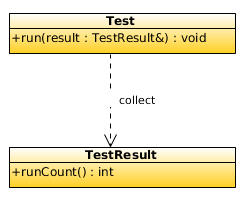
\includegraphics[width=0.4\textwidth]{figures/xunit/test-result.png}
\caption{聚集参数:收集测试结果}
 \label{fig:test-tree}
\end{figure}

\subsection{统计用例数目}

\ascii{TestResult::runCount}在运行时,通过监听接口统计测试用例的数目。事实上,也可以遍历用例树,直接统计测试用例的数目。构造一个失败的用例,观察如何统计测试用例数目。

\begin{leftbar}
 \begin{c++}[caption={\ttfamily{test/mars/core/TestSuiteSpec.cc}}]
#include <gtest/gtest.h>
#include "mars/core/TestCase.h"
#include "mars/core/TestSuite.h"
#include "mars/core/TestResult.h"

namespace {
  struct TestSuiteSpec : testing::Test {
    void run(::Test& test) {
      test.run(result);
    }

    int countTestCases(::Test& test) {
      return test.countTestCases();
    }

  protected:
    TestResult result;
  };
}

TEST_F(TestSuiteSpec, run_multi_test_cases_using_test_suite) {
  TestSuite suite;
  suite.add(new TestCase);
  suite.add(new TestCase);

  run(suite);

  ASSERT_EQ(2, countTestCases(suite));
}
 \end{c++}
\end{leftbar}

\subsubsection{通过编译}

\ascii{TestResult}维护了一个计数器,负责计数器初始化,累计操作数的职责。

\begin{leftbar}
 \begin{c++}[caption={\ttfamily{include/mars/core/Test.h}}]
#include <string>

struct Test {
  explicit Test(const std::string& name = "");
  virtual ~Test() {}

  const std::string& getName() const;

  virtual int countTestCases() const = 0;
  virtual void run() = 0;

private:
  std::string name;
};
 \end{c++}
\end{leftbar}

\ascii{TestCase::countTestCases}覆写行为直接返回\ascii{1}。

\begin{leftbar}
 \begin{c++}[caption={\ttfamily{src/mars/core/TestCase.cc}}]
int TestCase::countTestCases() const {
  return 1;
}
 \end{c++}
\end{leftbar}

\ascii{TestSuite::countTestCases}覆写行为类似于\ascii{reduce}操作。

\begin{leftbar}
 \begin{c++}[caption={\ttfamily{src/mars/core/TestSuite.cc}}]
int TestSuite::countTestCases() const {
  auto num = 0;
  foreach([&num](auto test) {
    num += test->countTestCases();
  });
  return num;
}
 \end{c++}
\end{leftbar}

至此,测试通过。

\end{content}

\section{异常处理}

\begin{content}

至此,框架不能处理任何异常逻辑。当用户调用\ascii{ASSERT\_EQ}失败时,抛出\ascii{AssertionError}异常,框架捕获该异常,标记该测试用例为\ascii{Failure};如果抛出其他异常,并被\ascii{mars}框架捕获,则标记该测试用例为\ascii{Error}。显式区分这两种异常类型,使得用户可以审查自己的测试用例,并修复失败的用例。

\subsection{断言失败}

当用例的断言失败,打印诸如如下详细信息,提示用户修复失败的用例。

\begin{leftbar}
 \begin{python}[caption={测试失败}]
/home/horance/code/cpp/mars/test/mars/core/TestCaseSpec.cc:33
expected value == 2, but got 0
 \end{python}
\end{leftbar}

接下来,构建失败的用例,在\ascii{runTest}时抛出异常\ascii{AssertionError},模拟断言失败的场景。

\begin{leftbar}
 \begin{c++}[caption={\ttfamily{test/mars/TestCaseSpec.cc}}]
#include "mars/core/TestCase.h"
#include "mars/except/AssertionError.h"

namespace {
  struct AssertionFailedTest : TestCase {
    void runTest() override {
      throw AssertionError("test.cpp:57", "expected value == 2, but got 3");
    }
  };
}

TEST_F(TestCaseSpec, throw_assertion_error_on_run_test) {
  AssertionFailedTest test;
  run(test);

  ASSERT_EQ(1, result.failCount());
}
 \end{c++}
\end{leftbar}

\subsubsection{异常类}

为了通过编译,引入\ascii{AssertionError}的异常类。它携带了断言失败处的文件名与行号\ascii{(src)},及其用例断言失败的具体原因\ascii{(msg)}。

\begin{leftbar}
 \begin{c++}[caption={\ttfamily{include/mars/except/AssertionError.h}}]
#include <string>
#include <exception>

struct AssertionError : std::exception {
  AssertionError(const std::string& src, const std::string& msg);
  ~AssertionError() noexcept = default;

  const char* what() const noexcept;

private:
  std::string msg;
};
 \end{c++}
\end{leftbar}

\ascii{AssertionError}实现如下。

\begin{leftbar}
 \begin{c++}[caption={\ttfamily{src/mars/except/AssertionError.cc}}]
#include "mars/except/AssertionError.h"

AssertionError::AssertionError(const std::string& src,
  const std::string& msg) : msg(src + "\n" + msg) {
}

const char* AssertionError::what() const noexcept {
  return msg.c_str();
}
 \end{c++}
\end{leftbar}

\subsubsection{通过编译}

\ascii{TestResult}新增名为\ascii{numOfFails}的计数器。

\begin{leftbar}
 \begin{c++}[caption={\ttfamily{include/mars/core/TestResult.h}}]
struct TestResult {
  TestResult();

  int failCount() const;
  void onFail();

private:
  int numOfFails;
};
 \end{c++}
\end{leftbar}

\subsubsection{通过链接}

\begin{leftbar}
 \begin{c++}[caption={\ttfamily{src/mars/core/TestResult.cc}}]
#include "mars/core/TestResult.h"

TestResult::TestResult() : numOfFails(0) {
}

int TestResult::failCount() const {
  return numOfFails;
}

void TestResult::onFail() {
  numOfFails++;
}
 \end{c++}
\end{leftbar}

\subsubsection{通过测试}

当执行\ascii{TestCase::run}时,捕获异常并通过调用\ascii{TestResult::fail},累加计数器\ascii{numOfFails}。

\begin{leftbar}
 \begin{c++}[caption={\ttfamily{src/mars/core/TestCase.cc}}]
#include "mars/core/TestCase.h"
#include "mars/core/TestResult.h"

void TestCase::run(TestResult& result) {
  setUp();

  try {
    runTest();
  } catch (const AssertionError&) {
    result.onFail();
  }

  tearDown();
}
 \end{c++}
\end{leftbar}

至此,测试通过。

\subsection{前置失败}

\ascii{TestCase}执行时,还未执行至\ascii{runTest}时,执行\ascii{setUp}可能就提前失败了。构建失败的用例,模拟前置失败的场景。

\begin{leftbar}
 \begin{c++}[caption={\ttfamily{test/mars/TestCaseSpec.cc}}]
namespace {
  struct AssertionFailedOnSetUpTest : TestCase {
    bool wasRun = false;

  private:
    void setUp() override {
      throw AssertionError("test.cpp:57", "expected value == 2, but got 3");
    }

    void runTest() override {
      wasRun = true;
    }
  };
}

TEST_F(TestCaseSpec, throw_assertion_error_on_setup) {
  AssertionFailedOnSetUpTest test;
  run(test);

  ASSERT_EQ(1, result.failCount());
  ASSERT_FALSE(test.wasRun);
}
 \end{c++}
\end{leftbar}

\subsubsection{通过测试}

为了通过测试,当执行\ascii{TestCase::setUp}时,捕获异常并通知\ascii{TestResult},然后立即终止用例的执行;毕竟环境没准备好,强制执行用例毫无意义。

\begin{leftbar}
 \begin{c++}[caption={\ttfamily{src/mars/core/TestCase.cc}}]
#include "mars/core/TestCase.h"
#include "mars/core/TestResult.h"

void TestCase::run(TestResult& result) {
  bool succ = false;
  try {
    setUp();
    succ = true;
  } catch (const AssertionError&) {
    result.onFail();
  }

  if (succ) {
    try {
      runTest();
    } catch (const AssertionError&) {
      result.onFail();
    }
  }

  tearDown();
}
 \end{c++}
\end{leftbar}

至此,测试通过。

\subsection{后置失败}

\ascii{TestCase::runBare}执行时,执行完\ascii{setUp, runTest}成功之后,接着执行\ascii{tearDown}时失败。构建失败的用例,模拟后置失败的场景。

\begin{leftbar}
 \begin{c++}[caption={\ttfamily{test/mars/TestCaseSpec.cc}}]
namespace {
  struct AssertionFailedOnTearDownTest : TestCase {
    void tearDown() override {
      throw AssertionError("test.cpp:57", "expected value == 2, but got 3");
    }
  };
}

TEST_F(TestCaseSpec, throw_assertion_error_on_tear_down) {
  AssertionFailedOnTearDownTest test;
  run(test);

  ASSERT_EQ(1, result.failCount());
}
 \end{c++}
\end{leftbar}

\subsubsection{通过测试}

当执行\ascii{TestCase::tearDown}时,捕获异常并通知\ascii{TestResult}。但是,无论\ascii{setUp, runTest}成败与否,\ascii{tearDown}都要强制执行,保证资源的安全释放。

\begin{leftbar}
 \begin{c++}[caption={\ttfamily{src/mars/core/TestCase.cc}}]
#include "mars/core/TestCase.h"
#include "mars/core/TestResult.h"

void TestCase::run(TestResult& result) {
  bool succ = false;
  try {
    setUp();
    succ = true;
  } catch (const AssertionError&) {
    result.onFail();
  }

  if (succ) {
    try {
      runTest();
    } catch (const AssertionError&) {
      result.onFail();
    }
  }

  try {
    tearDown();
  } catch (const AssertionError&) {
    result.onFail();
  }
}
 \end{c++}
\end{leftbar}

至此,测试通过。

\subsection{异常与错误}

当抛出\ascii{AssertionError},称之为\ascii{Failure};当抛出其他异常,称之为\ascii{Error}。构建失败的用例,模拟其他异常抛出的场景。

\begin{leftbar}
 \begin{c++}[caption={\ttfamily{test/mars/TestCaseSpec.cc}}]
namespace {
  struct StdExceptionTest : TestCase {
    void runTest() override {
      throw std::exception();
    }
  };
}

TEST_F(TestCaseSpec, throw_std_exception_on_run_test) {
  StdExceptionTest test;
  run(test);

  ASSERT_EQ(0, result.failCount());
  ASSERT_EQ(1, result.errorCount());
}
 \end{c++}
\end{leftbar}

\subsubsection{捕获异常}

当执行\ascii{TestCase::runTest}时,捕获\ascii{std::exception}异常,并通知\ascii{TestResult::error}累加计数器。

\begin{leftbar}
 \begin{c++}[caption={\ttfamily{src/mars/core/TestCase.cc}}]
#include "mars/core/TestCase.h"
#include "mars/core/TestResult.h"

void TestCase::run(TestResult& result) {
  bool succ = false;
  try {
    setUp();
    succ = true;
  } catch (const AssertionError&) {
    result.onFail();
  }

  if (succ) {
    try {
      runTest();
    } catch (const AssertionError&) {
      result.onFail();
    } catch (const std::exception&) {
      result.onError();
    }
  }

  try {
    tearDown();
  } catch (const AssertionError&) {
    result.onFail();
  }
}
 \end{c++}
\end{leftbar}

\subsubsection{错误计数器}

增加\ascii{TestResult::errorCount}的成员函数,及其相应的计数器\ascii{numOfErrors}。

\begin{leftbar}
 \begin{c++}[caption={\ttfamily{include/mars/core/TestResult.h}}]
struct TestResult {
  TestResult();

  int failCount() const;
  int errorCount() const;

  void onFail();
  void onError();

private:
  int numOfFails;
  int numOfErrors;
};
 \end{c++}
\end{leftbar}

\subsubsection{通过链接}

\begin{leftbar}
 \begin{c++}[caption={\ttfamily{src/mars/core/TestResult.cc}}]
#include "mars/core/TestResult.h"

TestResult::TestResult()
  : numOfFails(0), numOfErrors(0) {
}

int TestResult::failCount() const {
  return numOfFails;
}

int TestResult::failCount() const {
  return numOfErrors;
}

void TestResult::onFail() {
  numOfFails++;
}

void TestResult::onError() {
  numOfErrors++;
}
 \end{c++}
\end{leftbar}

至此,测试通过。

\subsection{未知错误}

当抛出其他未知的异常,测试框架需要捕获,并标记为\ascii{Error},提示用户被测系统存在严重的漏洞。

\begin{leftbar}
 \begin{c++}[caption={\ttfamily{test/mars/TestCaseSpec.cc}}]
namespace {
  struct UnknownExceptionTest : TestCase {
    void runTest() override {
      throw std::out_of_range("overflow");
    }
  };
}

TEST_F(TestCaseSpec, throw_unknown_exception_on_run_test) {
  UnknownExceptionTest test;
  run(test);

  ASSERT_EQ(0, result.failCount());
  ASSERT_EQ(1, result.errorCount());
}
 \end{c++}
\end{leftbar}

\subsubsection{捕获异常}

当执行\ascii{TestCase::runTest}时,捕获未知的异常,并通知\ascii{TestResult::error}累加计数器。

\begin{leftbar}
 \begin{c++}[caption={\ttfamily{src/mars/core/TestCase.cc}}]
#include "mars/core/TestCase.h"
#include "mars/core/TestResult.h"

void TestCase::run(TestResult& result) {
  bool succ = false;
  try {
    setUp();
    succ = true;
  } catch (const AssertionError&) {
    result.onFail();
  }

  if (succ) {
    try {
      runTest();
    } catch (const AssertionError&) {
      result.onFail();
    } catch (const std::exception&) {
      result.onError();
    } catch (...) {
      result.onError();
    }    
  }

  try {
    tearDown();
  } catch (const AssertionError&) {
    result.onFail();
  }
}
 \end{c++}
\end{leftbar}

测试通过。

\subsection{完备的异常处理}

依次构建测试用例,小步快走,驱动出完备的异常处理逻辑。

\begin{leftbar}
 \begin{c++}[caption={\ttfamily{src/mars/core/TestCase.cc}}]
#include "mars/core/TestCase.h"
#include "mars/core/TestResult.h"

void TestCase::run(TestResult& result) {
  bool succ = false;
  try {
    setUp();
    succ = true;
  } catch (const AssertionError&) {
    result.onFail();
  } catch (const std::exception&) {
    result.onError();
  } catch (...) {
    result.error();
  }

  if (succ) {
    try {
      runTest();
    } catch (const AssertionError&) {
      result.onFail();
    } catch (const std::exception&) {
      result.error();
    } catch (...) {
      result.error();
    }
  }

  try {
    tearDown();
  } catch (const AssertionError&) {
    result.fail();
  } catch (const std::exception&) {
    result.error();
  } catch (...) {
    result.error();
  }
}

void TestCase::run(TestResult& result) {
  result.run();
  runBare(result);
}
 \end{c++}
\end{leftbar}

至此,\ascii{TestCase::runBare}的实现,不仅存在重复逻辑,而且异常臃肿,异常丑陋。此时不重构,更待何时。

\subsubsection{消除重复}

观察\ascii{TestCase::setUp, TestCase::runTest, TestCase::tearDown}之间的共性,它们拥有相同的函数签名,可以使用指向成员函数的指针挖掘它们的共性。

\begin{leftbar}
 \begin{c++}
using Method = void(TestCase::*)();
 \end{c++}
\end{leftbar}

提取公共函数\ascii{TestCase::protect},它返回\ascii{bool}类型。

\begin{leftbar}
 \begin{c++}[caption={\ttfamily{src/mars/core/TestCase.cc}}]
#include "mars/core/TestCase.h"
#include "mars/core/TestResult.h"

using Method = void(TestCase::*)();

bool TestCase::protect(TestResult& result, Method method) {
  bool succ = false;
  try {
    (this->*method)();
    succ = true;
  } catch (const AssertionError&) {
    result.onFail();
  } catch (const std::exception&) {
    result.onError();
  } catch (...) {
    result.onError();
  }
  return succ;
}

void TestCase::run(TestResult& result) {
  if (protect(result, &TestCase::setUp)) {
    protect(result, &TestCase::runTest);
  }
  protect(result, &TestCase::tearDown);
}
 \end{c++}
\end{leftbar}

\end{content}

\section{解耦合}

\begin{content}

分析\ascii{TestCase}实现,\ascii{TestCase::setUp, TestCase::runTest, TestCase::tearDown}宿主于\ascii{TestCase},而异常处理逻辑主要宿主于\ascii{TestResult}。根据迪米特法则,这段异常处理的逻辑应搬迁至\ascii{TestResult};当捕获异常后,直接更新到自己的私有数据域,使得\ascii{TestResult::onRun, TestResult::onFail, TestResult::onError}等监听接口完全私有化。

但是,\ascii{TestResult}如何调用到\ascii{TestCase::setUp, TestCase::runTest, TestCase::tearDown}成员函数呢?此时似乎陷入窘境,因为\ascii{TestCase}与\ascii{TestResult}之间的耦合太过紧密,拆分显得不是那么容易。

因此,解除\ascii{TestCase}与\ascii{TestResult}之间的耦合迫在眉睫。

\subsection{引入TestCaseFunctor}

引入\ascii{TestCaseFunctor}的抽象类型,让\ascii{TestResult}依赖于\ascii{TestCaseFunctor}的抽象类型,而非具体的\ascii{TestCase}。一方面,它可以获知\ascii{TestCase}的名字;另一方面它可以调用\ascii{TestCase::setUp}, 或\ascii{TestCase::runTest}, 或\ascii{TestCase::tearDown}。

\begin{leftbar}
 \begin{c++}[caption={\ttfamily{include/mars/core/internal/TestCaseFunctor.h}}]
#include <string>

struct TestCaseFunctor {
  virtual ~TestFunctor() {}

  virtual const std::string& getTestName() const = 0;  
  virtual bool operator()() const = 0;
};
 \end{c++}
\end{leftbar}

\subsubsection{实现TestCaseFunctor}

\ascii{TestCase::Functor}是\ascii{TestCaseFunctor}背后运行的基石,它封装了\ascii{TestCase::setUp, TestCase::runTest, TestCase::tearDown}的调用。

一方面,\ascii{TestCase::Functor}被声明为\ascii{private},屏蔽外界的访问;另一方面,它能够调用\ascii{TestCase}的私有成员,例如私有的\ascii{TestCase::getTestName}。

\begin{leftbar}
 \begin{c++}[caption={\ttfamily{include/mars/core/TestCase.h}}]
#include "mars/core/Test.h"

struct TestCase : Test {
  using Test::Test;

private:
  int countTestCases() const override;
  void run(TestResult&) override;

private:
  virtual void setUp() {}
  virtual void runTest() {}
  virtual void tearDown() {}

private:
  struct Functor;
  std::string name;
};
 \end{c++}
\end{leftbar}

在\ascii{TestCase.cc}的实现文件中,实现\ascii{TestCase::Functor}的逻辑。

\begin{leftbar}
 \begin{c++}[caption={\ttfamily{src/mars/core/TestCase.cc}}]
#include "mars/core/TestCase.cc"
#include "mars/core/internal/TestCaseFunctor.h"

namespace {
  struct Functor : TestCaseFunctor {
    using Method = void(TestCase::*)();

    Functor(TestCase* self, Method method)
      : self(self), method(method) {
    }

  private:
    const std::string& getTestName() const override {
      return self->getName();
    }

    bool operator()() const override {
      (self->*method)();
      return true;
    }

  private:
    TestCase* self;
    Method method;
  };
}

void TestCase::run(TestResult& result) {
  if (result.protect(Functor(this, &TestCase::setUp, "in the setUp"))) {
    result.protect(Functor(this, &TestCase::runTest, "in the runTest"));
  }
  result.protect(Functor(this, &TestCase::tearDown, "in the tearDown"));
}
 \end{c++}
\end{leftbar}

其中,\ascii{TestResult::protect}将搬迁异常处理的逻辑,使其各司其职,留待还需处理。

\subsubsection{改善表达力}

可以引入一个宏定义,改善\ascii{TestResult::protect}调用的表达力。不忘初心,\ascii{TestCase::runBare}的算法主干回归至最开始的简单逻辑,但它已经具备完备的异常处理机制。

\begin{leftbar}
 \begin{c++}[caption={\ttfamily{src/mars/core/TestCase.cc}}]
#define PROTECT(method) \
    result.protect(Functor(this, &TestCase::method, "in the "#method))

void TestCase::run(TestResult& result) {
  if (PROTECT(setUp)) {
    PROTECT(runTest);
  }
  PROTECT(tearDown);
}
 \end{c++}
\end{leftbar}

\subsection{搬迁异常逻辑}

接下来,运用迪米特法则,将异常处理的逻辑\ascii{TestCase::protect}搬迁到\ascii{TestResult}。此外,\ascii{TestResult::protect}依赖与\ascii{TestCaseFunctor}的抽象类型,而非具体的\ascii{TestCase},实现了\ascii{TestResult}对\ascii{Test}的解耦。

\begin{leftbar}
 \begin{c++}[caption={\ttfamily{src/mars/core/TestResult.cc}}]
#include "mars/core/internal/TestCaseFunctor.h"

bool TestResult::protect(const TestCaseFunctor& f) {
  try {
    return f();
  } catch (const AssertionError&) {
    onFail();
  } catch (const std::exception&) {
    onError();
  } catch (...) {
    onError();
  }
  return false;
}
 \end{c++}
\end{leftbar}

\subsection{传递异常}

为了给用户提供更为精准的异常信息,需要将其存储于\ascii{TestResult}。首先提取\ascii{TestFailure}的概念,将所有异常信息打包到一起。

\begin{leftbar}
 \begin{c++}[caption={\ttfamily{include/mars/except/TestFailure.h}}]
#include <string>

struct TestFailure {
  TestFailure(const std::string& name, const std::string& msg, bool failure);

  const std::string& getTestName() const;
  const std::string& getExceptionMsg() const;
  bool isFailure() const;
  bool isError() const;

private:
  std::string name;
  std::string msg;
  bool failure;
};

 \end{c++}
\end{leftbar}

\ascii{TestFailure}是一个实体类,实现非常简单。

\begin{leftbar}
 \begin{c++}[caption={\ttfamily{src/mars/except/TestFailure.cc}}]
#include "mars/except/TestFailure.h"

TestFailure::TestFailure
  ( const std::string& name, const std::string& msg, bool failure)
  : name(name), msg(msg), failure(failure) {
}

const std::string& TestFailure::getTestName() const {
  return name;
}

const std::string& TestFailure::getExceptionMsg() const {
  return msg;
}

bool TestFailure::isFailure() const {
  return failure;
}

bool TestFailure::isError() const {
  return !failure;
}
 \end{c++}
\end{leftbar}

\subsubsection{存储异常}

在\ascii{TestResult}存储异常列表,需要管理其动态内存。

\begin{leftbar}
 \begin{c++}[caption={\ttfamily{include/mars/core/TestResult.h}}]
struct TestResult {
  TestResult();
  ~TestResult();

  bool protect(const TestFunctor&);

  int runCount() const;
  int failCount() const;
  int errorCount() const;

private:
  void onFail();
  void onError();

private:
  int numOfRuns;
  int numOfFails;
  int numOfErrors;

  std::vector<TestFailure*> failures;
};
 \end{c++}
\end{leftbar}

实现文件中,主要完成\ascii{TestFailure}的构造,及其动态内存的管理。

\begin{leftbar}
 \begin{c++}[caption={\ttfamily{src/mars/core/TestResult.cc}}]
TestResult::~TestResult() {
  for (auto f : failures) {
    delete f;
  }
}

void TestResult::addFailure(TestFailure* f) {
  failures.push_back(f);
}

namespace {
  TestFailure* failure(
      const TestFunctor& f,
      const char* why,
      const char* where,
      const char* what) {
    return new TestFailure
      (f.getTestName(), std::string(why) + where + what, true);
  }

  TestFailure* error(
      const TestFunctor& f,
      const char* why,
      const char* where,
      const char* what) {
    return new TestFailure
      (f.getTestName(), std::string(why) + where + what, false);
  }
}

bool TestResult::protect(const TestFunctor& f, const char* where) {
  try {
    return f();
  } catch (const AssertionError& e) {
    onFail();
    addFailure(failure(f, "assertion fail", where, e.what()));
  } catch (const std::exception& e) {
    onError();
    addFailure(error(f, "uncaught std::exception", where, e.what()));
  } catch (...) {
    onError();
    addFailure(error(f, "uncaught unknown exception", where, ""));
  }
  return false;
}
 \end{c++}
\end{leftbar}

\end{content}